\section{YOLOv3}  \label{sec:yolov3}

The YOLOv3 model is the next incremental improvement of the YOLO family after YOLO9000. The YOLOv3 model is introduced in 2018 \cite{yolov3_2018}, which consists of four main minor changes to the YOLOv2 architecture. 

The first change is replacing the softmax function with independent logistics for the classifier. While the softmax function requires the sum of all class probabilities to 1, independent logistics consider each class independently, and the probability of any two class do not affect one another \cite{yolov3_2018}. This improves the model's classifier from a multi-class classifier to a multi-class and multi-label classifier. That is, when the classifier is multi-class and multi-label, there is no competition between labels. For example, if a pedestrian is a woman and the supported label include both "pedestrian" and "women", then when using an independent logistic classifier, the probability for both label should be high for this object, while the softmax classifier will only give high probability to one of the two labels.

While the format of the predicted bounding in YOLOv3 is the same as YOLOv2 (Figure \ref{fig:yolov2_bbox}), the calculation of the confidence score and loss function are different compared to YOLOv2. This is the second change the YOLOv3 proposed compared to YOLOv2. The YOLOv3 predicts the bounding box's confidence (objectness) score is predicted using a logistic regression \cite{yolov3_2018}. This is trained by setting the confidence score of the bounding box anchor to 1 if the anchor box has the highest IoU score with the ground-truth box compared to other anchors. Additionally, during training, any anchor box that has an IoU score of more than 0.5 with a ground-truth box but the IoU score is not the highest among anchor boxes for this object, then that anchor box will not contribute to the loss function. If the model does not predict a bounding box anchor for a ground-truth object, the objectness loss will increase and contribute no effect to localization loss and classification loss. Similar to YOLOv1 and YOLOv2, YOLOv3 also optimizes for sum-square error loss, which combines the localization, classification, and objectness loss into one metric. 

The third change is detection at 3 different scales per cell. At each cell, the model predicts $B$ bounding boxes for each feature map scale, i.e., the current feature map and two upscaled feature maps. Assume we divide the image into $S \times S$ cells and the dataset is COCO 80 labels, then at each scale, the model predict $S \times S \times [3_{bbox} * (4 + 1 + 80)]$, thus the model generate a $S \times N \times [3_{scale} * 3_{bbox} * (4 + 1 + 80)]$ \cite{yolov3_2018}. The YOLOv3 model predicts 9 anchor boxes per cell. These 9 anchor boxes are chosen using the k-means clustering algorithm and divided into each scale evenly. For example, the YOLOv3 model trained for the COCO dataset will have the following 9 anchor boxes:
\begin{align*}
    Scale-1: &[(10 \times 13), (16 \times 30), (33 \times 23)] \\
    Scale-2: &[(30 \times 61), (62 \times 45), (59 \times 119)] \\
    Scale-3: &[(116  \times  90), (156  \times  198), (373  \times  326)]    
\end{align*}
    
The fourth change is the feature extractor. Inspired by Darknet-19 and ResNet, the author proposed a new CNN architecture, namely Darknet-53. The overall architechture of Darknet-53 is shown in Firgure \ref{fig:darknet53_archite}. The network consists of 53 convolutional layers, $3 \times 3$ or $1 \times 1$ convolutional layers, and using shortcut connections \cite{yolov3_2018}. The shortcut connections are introduced in the ResNet model and are used to skip over certain convolutional layers based on certain conditions, which improve the runtime and address problems with high-depth networks \cite{resnet_2016}. The Darknet-53 is two times faster than the ResNet-152 model while preserving the model's accuracy. Other than the loss computation method, the Darknet-53 training is the same as YOLOv2, which includes batch normalization, multi-scale training, and data augmentation.
\begin{figure}[!ht]
    \centering
    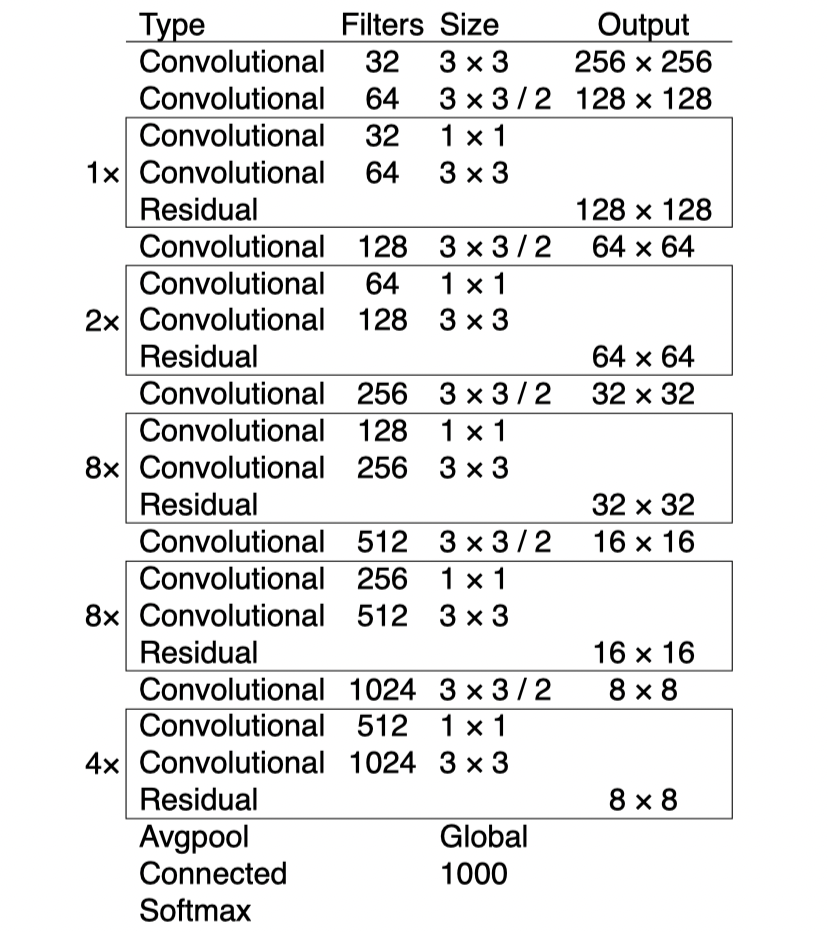
\includegraphics[width=3in]{figures/darknet53_archite.png}
    \caption{Darknet-53 architecture \cite{yolov3_2018}} 
    \label{fig:darknet53_archite}
\end{figure}